%-------------------------------------------
% En-tête type de document pour le projet PLD
% Il suffit de remplir le input ligne 45
%-------------------------------------------

\documentclass[a4paper]{article}

\usepackage[utf8]{inputenc}   
\usepackage[top=2cm, bottom=2cm, left=2cm, right=2cm]{geometry}
\usepackage{ucs}
% Reconnaitre les caratères accentués dans le source.
\usepackage[T1]{fontenc} 
\usepackage{lmodern}
\usepackage[francais]{babel}
% Insertion d'images
\usepackage{graphicx}
% Utilisation du symbole EURO
\usepackage{eurosym}

\begin{document}

%------------------------------------- Page de titre
\begin{titlepage}
~ 
\vfill
	\begin{center}
		\begin{Huge}
		Projet Système d'Information Urbanisé \& SOA : Compte Rendu\\
		\end{Huge} 
\vfill
		\textbf{Hexanome 4111 :} 
		\\Quentin \bsc{Calvez}, Matthieu \bsc{Coquet}, 
		\\Jan \bsc{Keromnes}, Alexandre \bsc{Lefoulon}, 
		\\Xavier \bsc{Sauvagnat, }Thaddée \bsc{Tyl},
		\\Tuuli \bsc{Tyrväinen}
\vfill		
		\begin{Large}
		Février 2012
		\end{Large}
\vfill
	\begin{tabular}{|c|c|c|c|c|}
 	 \hline
   Destinataire & Version & Etat & Dernière révision & Equipe \\
   \hline
   Client & 1 & Validé & \today & H4111 \\
   \hline
	\end{tabular}
	\end{center}
\vfill
\end{titlepage}
%----------------------------------------------------
%--------------------------------- Table des matières
\newpage
\tableofcontents
\newpage
%----------------------------------------------------

%------------------- Insertion du contenu du document

%Corps du document :
%\setlength{\parindent}{1cm}    

\section{Conception d'ensemble de l'architecture applicative}

\subsection{Analyse des modèles conceptuels proposés}

\subsection{Établissement des diagrammes de séquences systèmes}

\subsection{Diagrammes d'activité}

\begin {center}
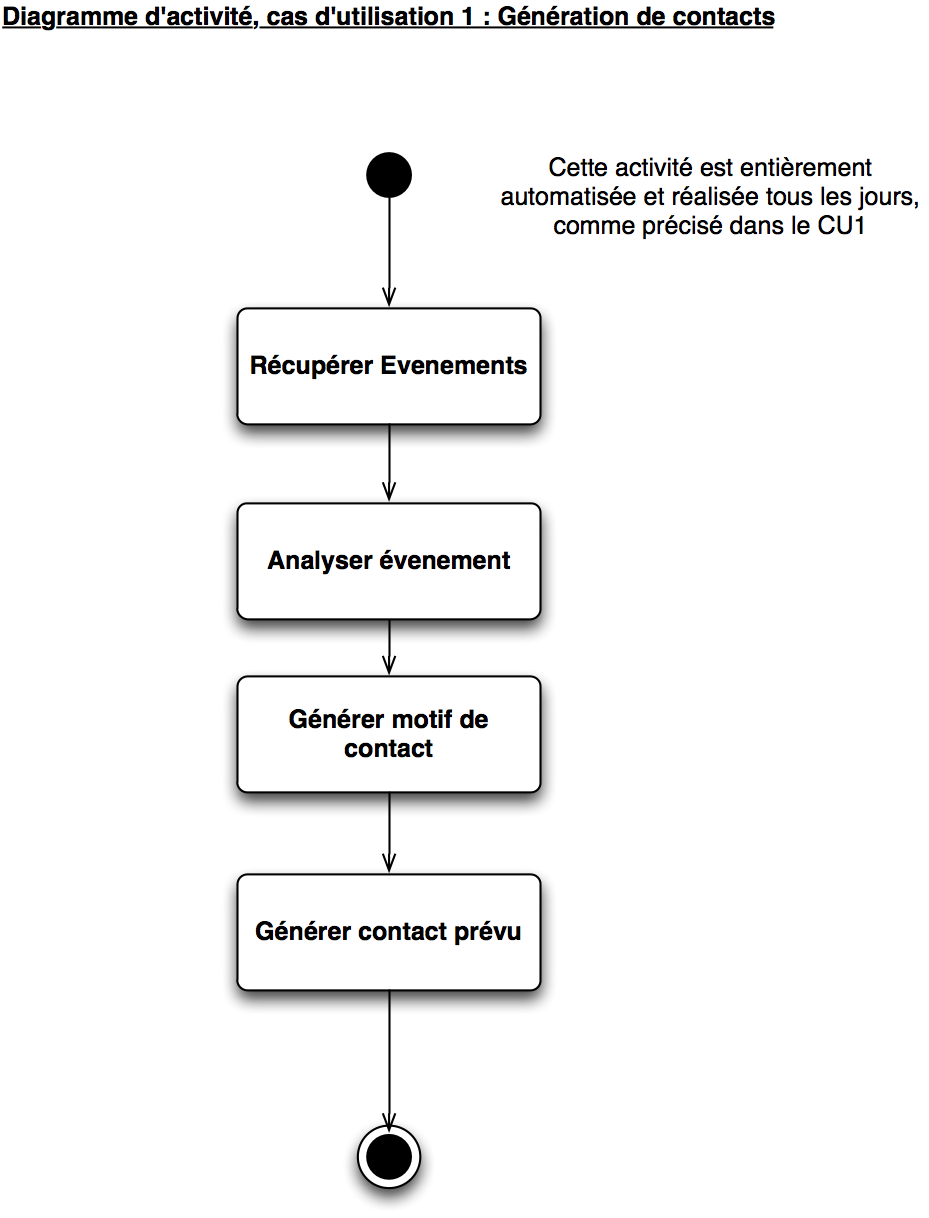
\includegraphics[width=\textwidth]{..\..\diagrammeActivite\DACU1.png}
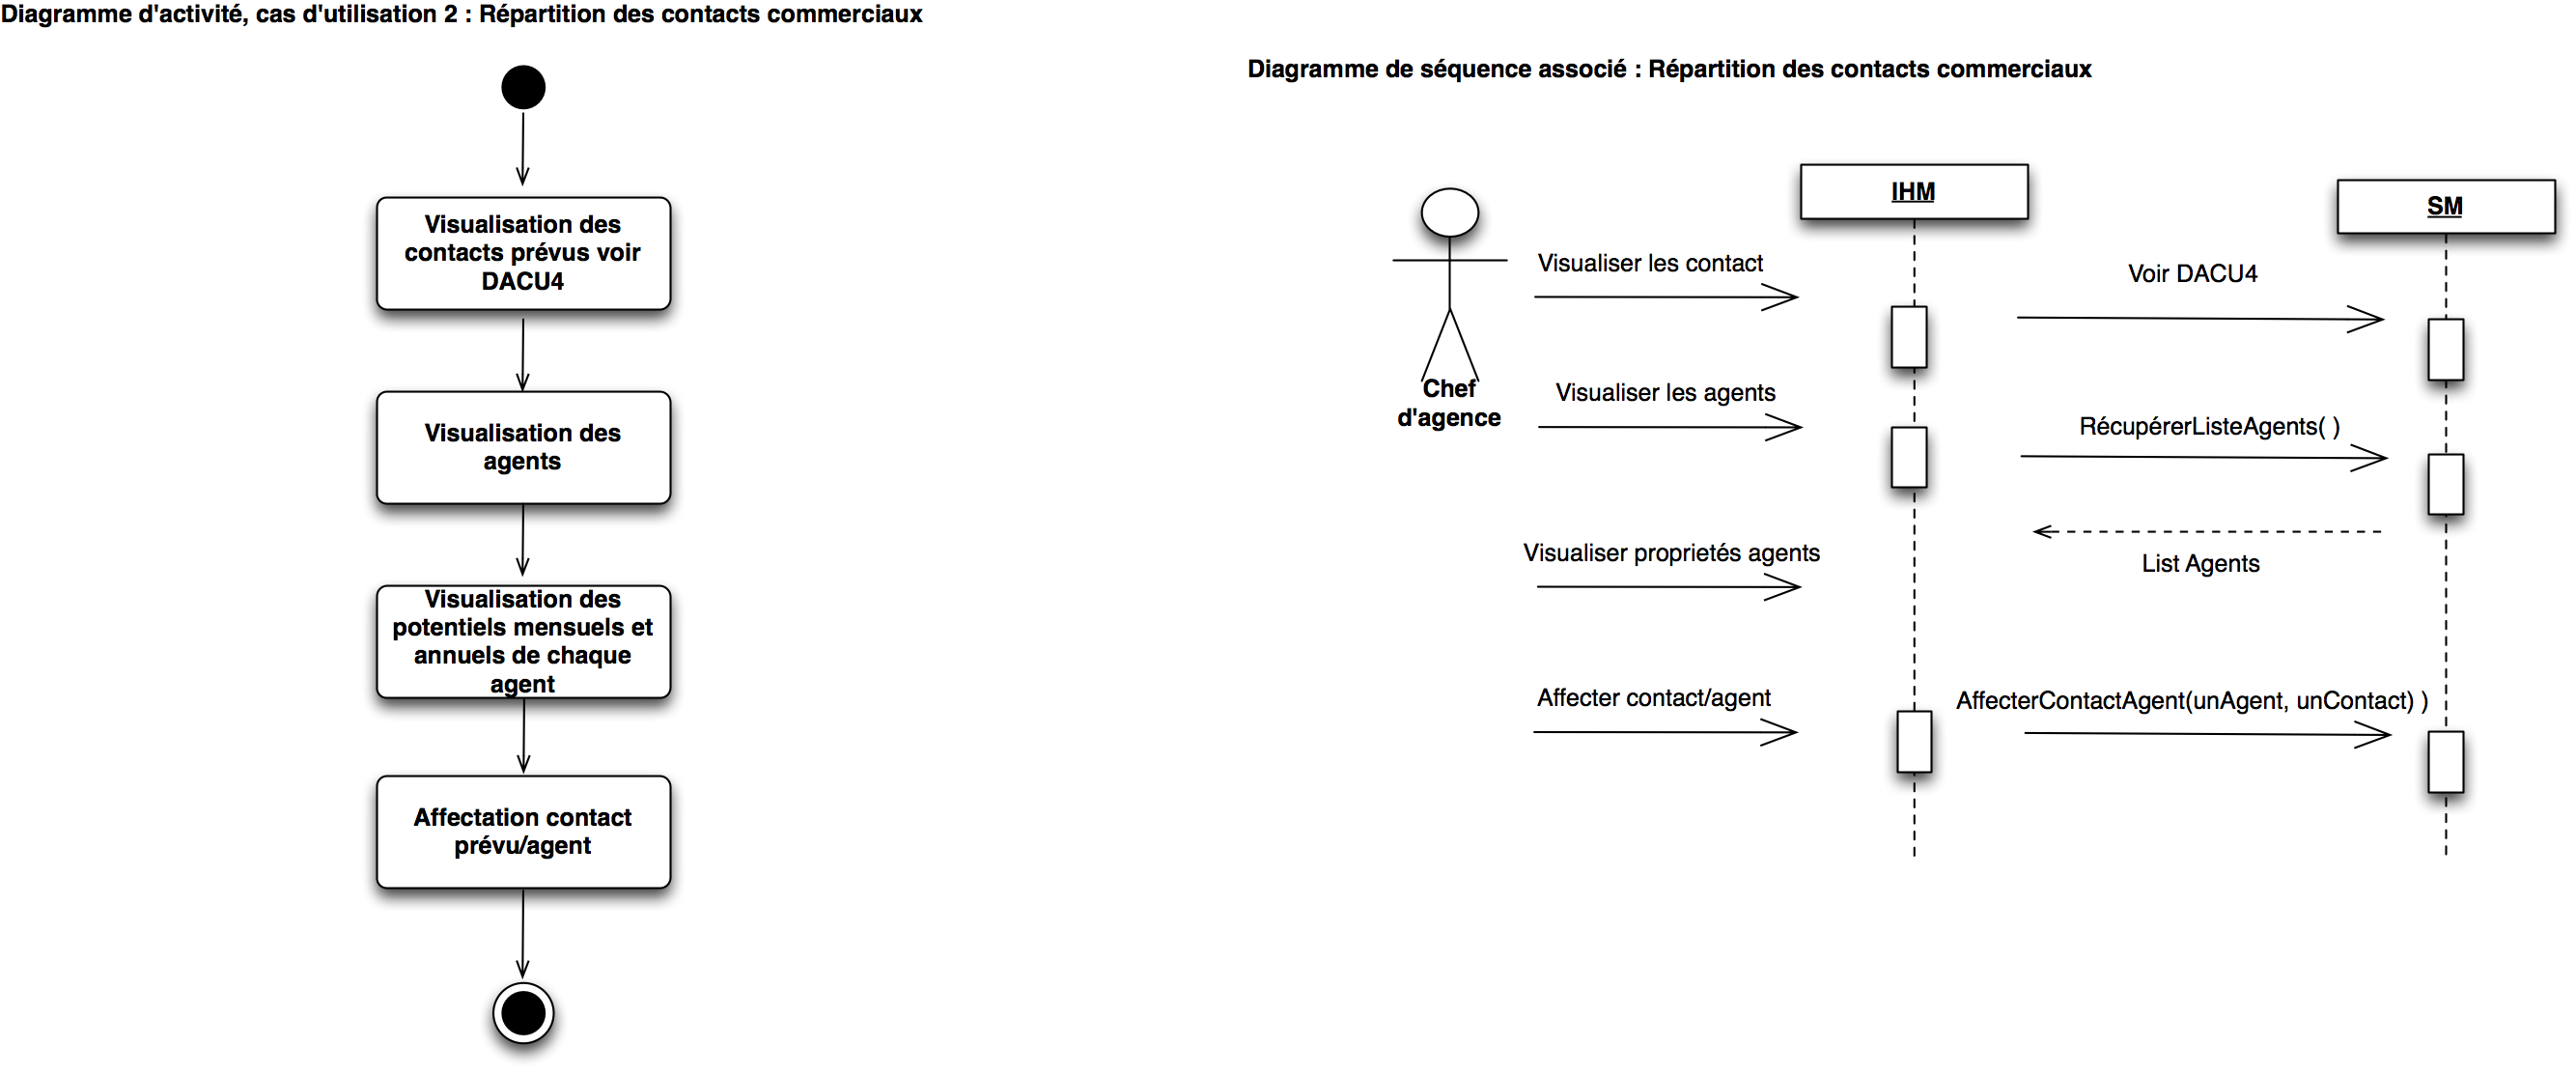
\includegraphics[width=\textwidth]{..\..\diagrammeActivite\DACU2.png}
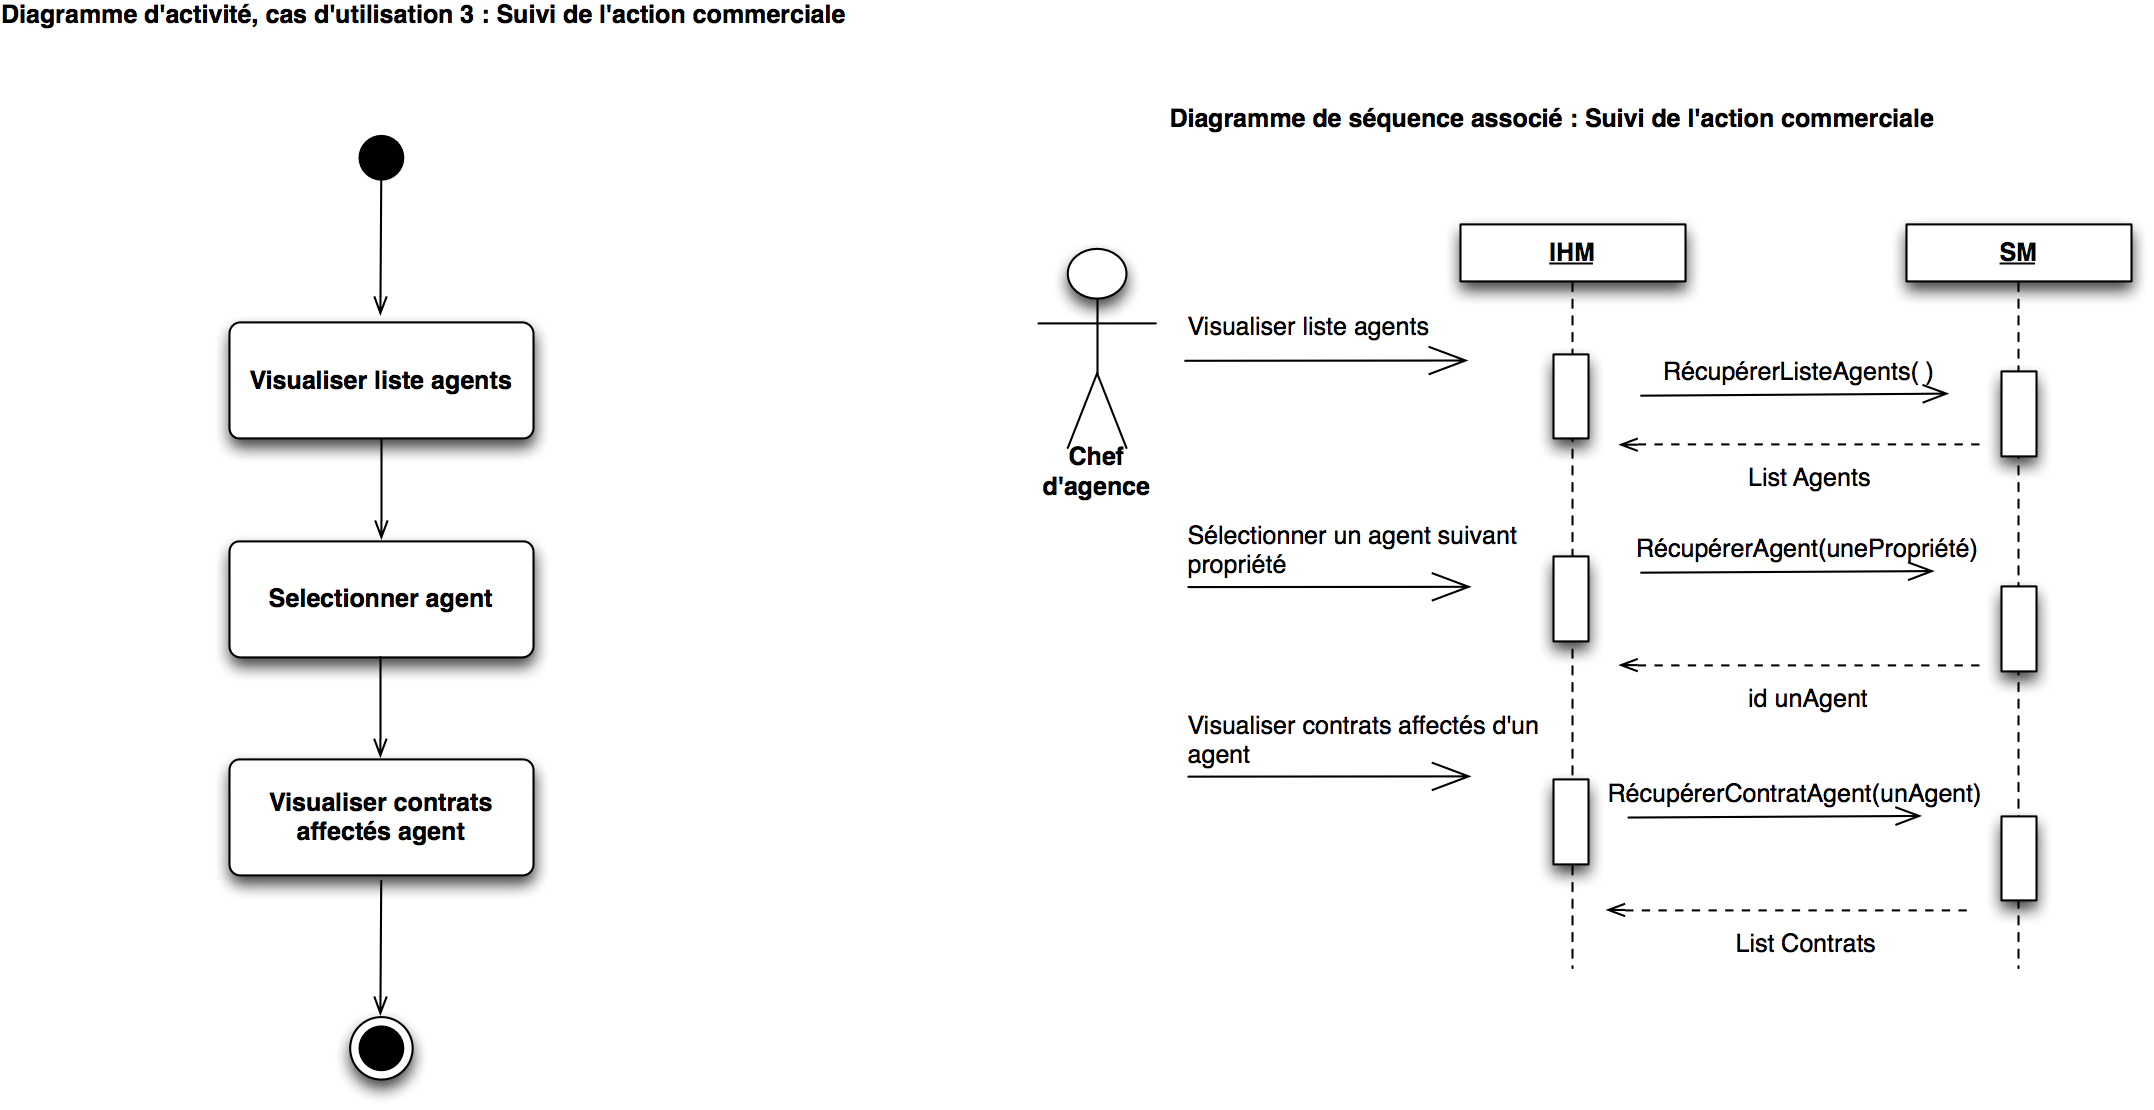
\includegraphics[width=\textwidth]{..\..\diagrammeActivite\DACU3.png}
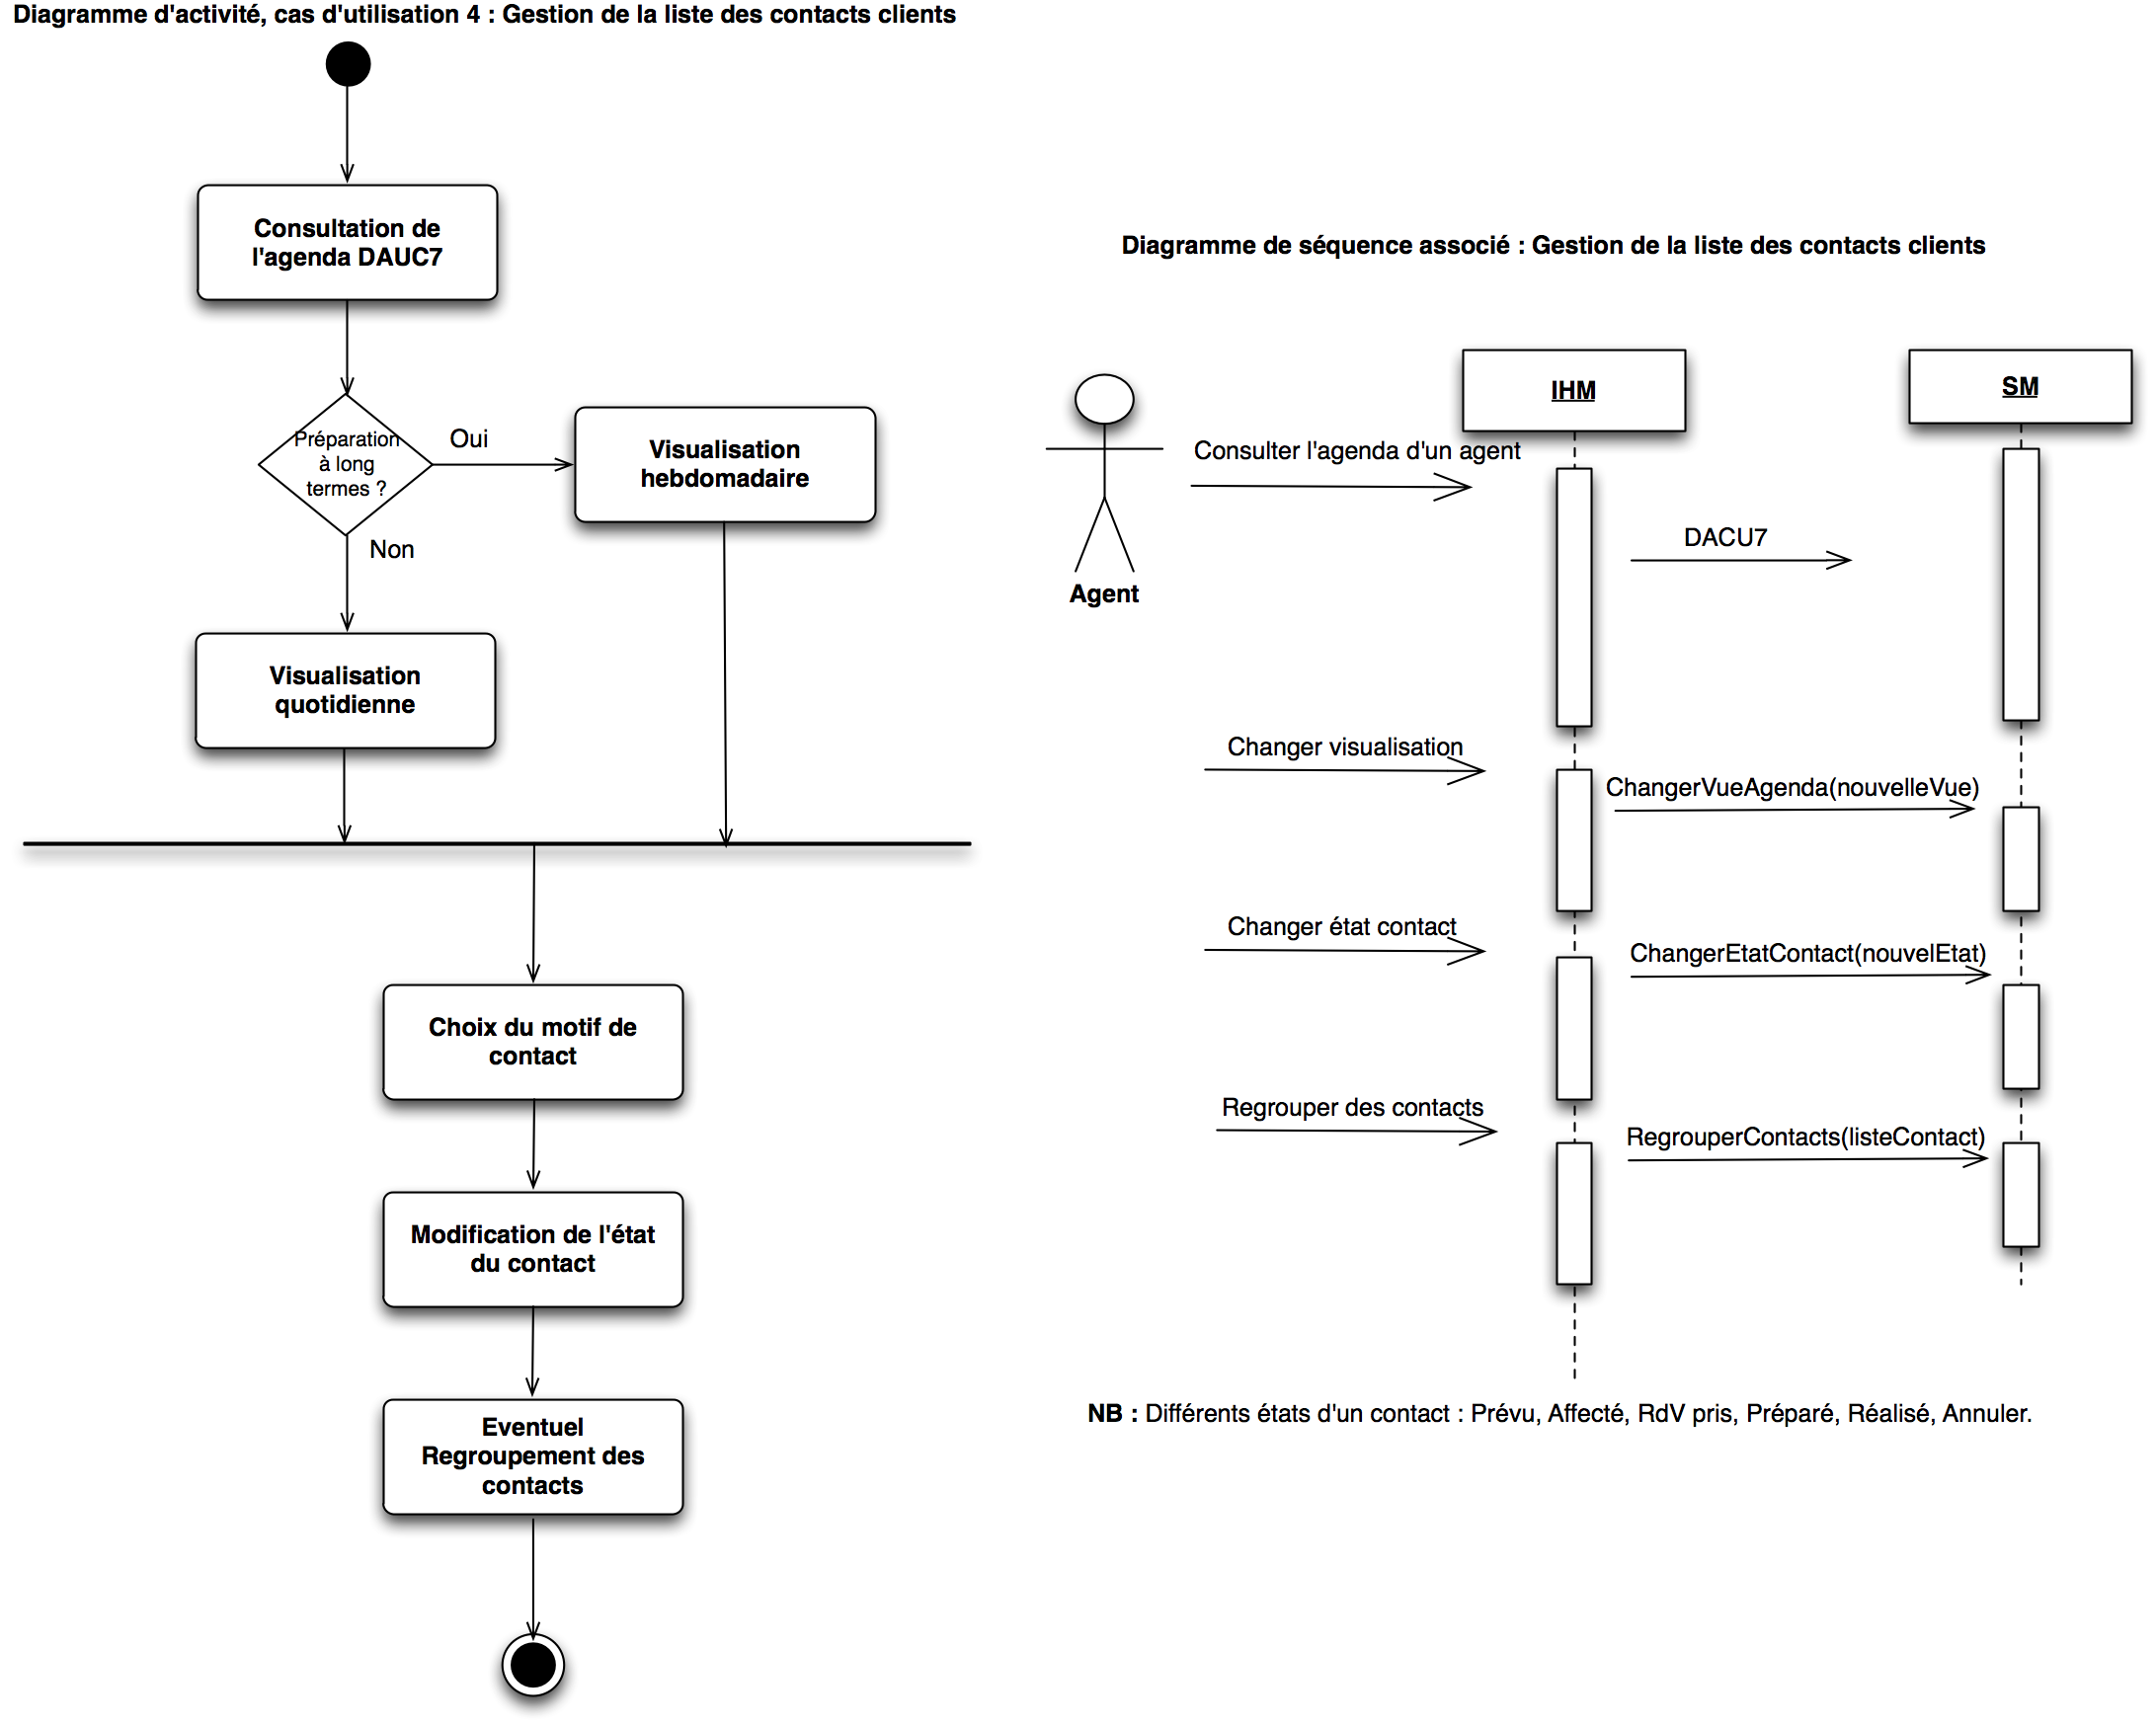
\includegraphics[width=\textwidth]{..\..\diagrammeActivite\DACU4.png}
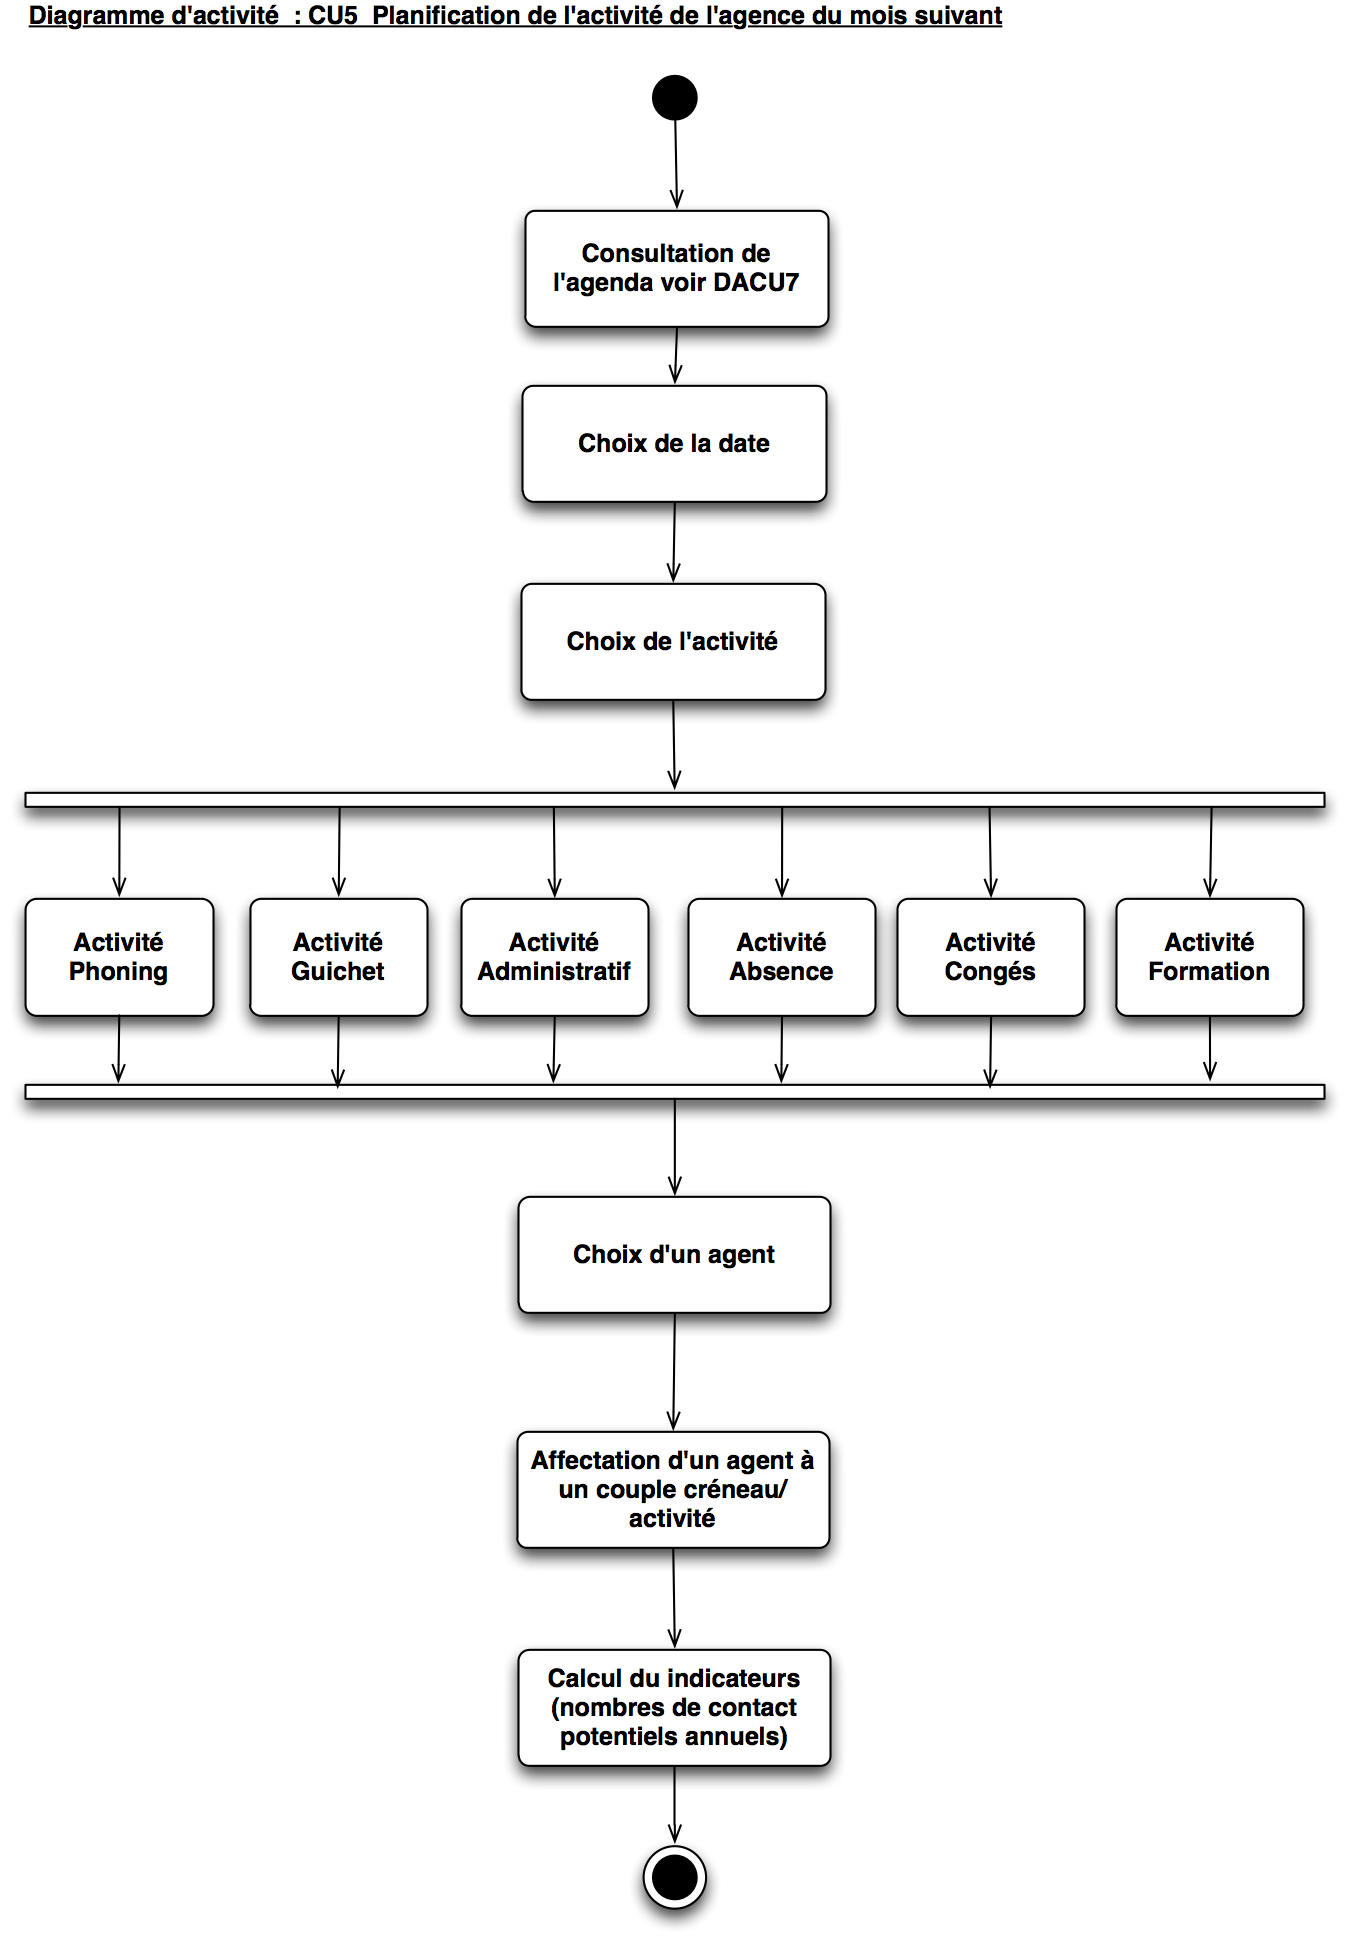
\includegraphics[width=\textwidth]{..\..\diagrammeActivite\DACU5.png}
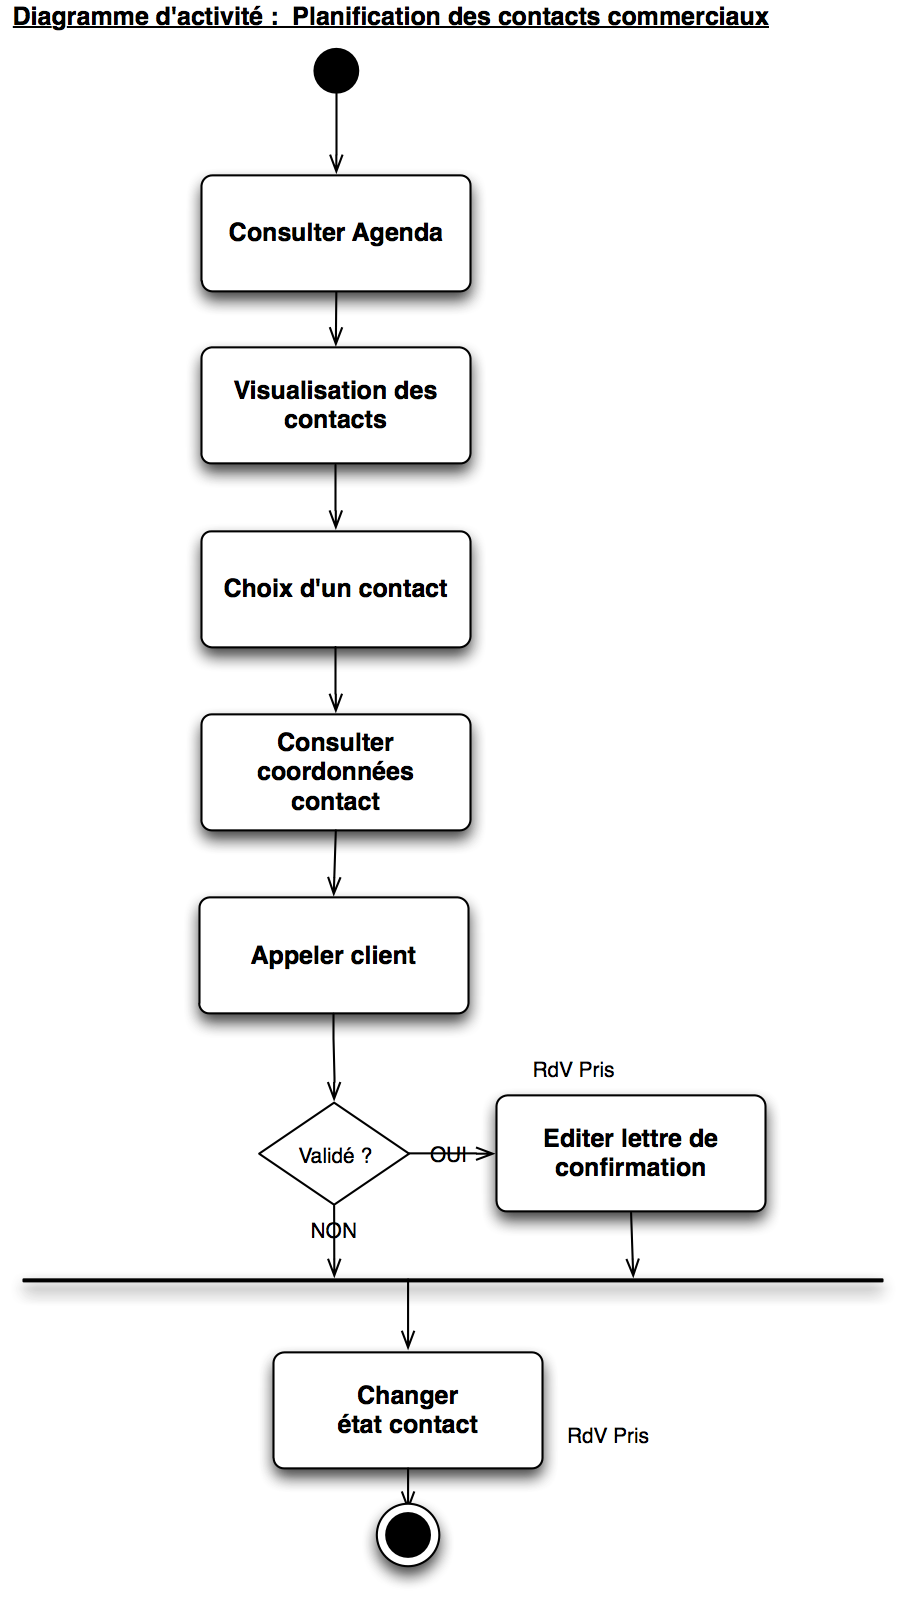
\includegraphics[width=\textwidth]{..\..\diagrammeActivite\DACU6.png}
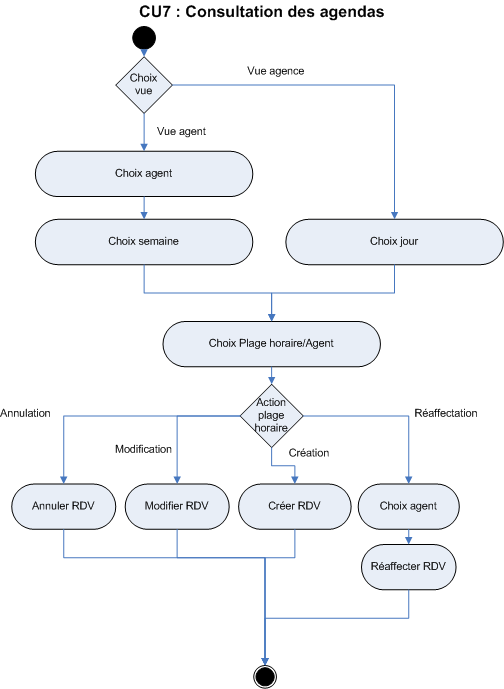
\includegraphics[width=\textwidth]{..\..\diagrammeActivite\DACU7.png}
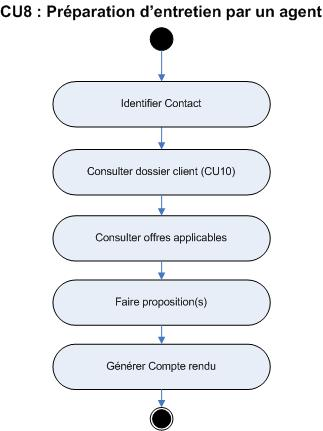
\includegraphics[width=\textwidth]{..\..\diagrammeActivite\DACU8.jpg}
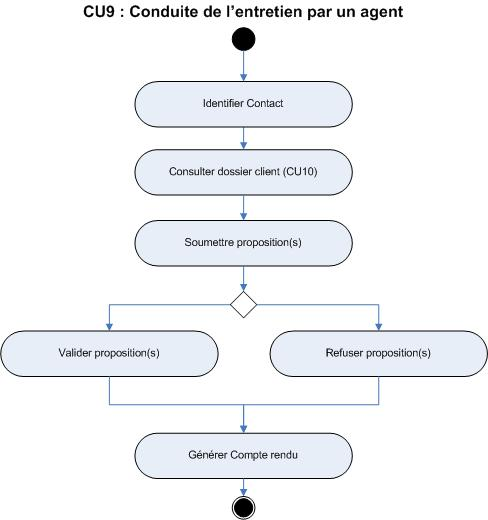
\includegraphics[width=\textwidth]{..\..\diagrammeActivite\DACU9.jpg}
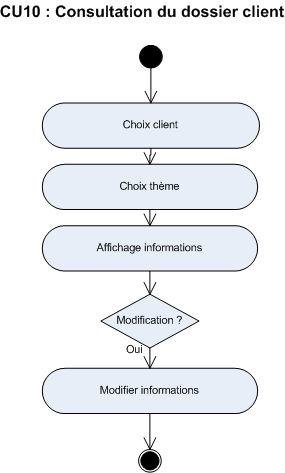
\includegraphics[width=\textwidth]{..\..\diagrammeActivite\DACU10.png}
\end {center}

\subsection{Blocs applicatifs}

\begin {center}
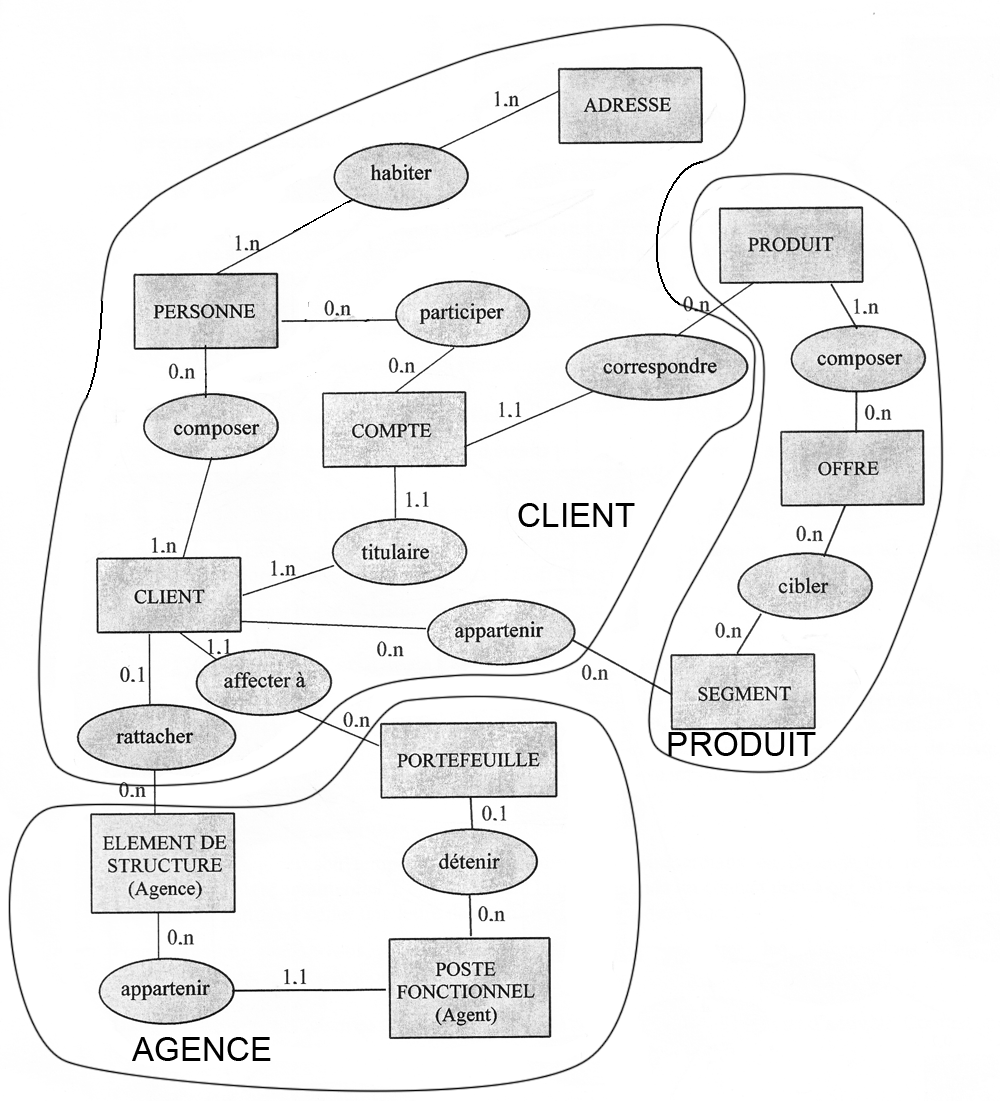
\includegraphics[width=\textwidth]{Decoupage MCD 1.png}
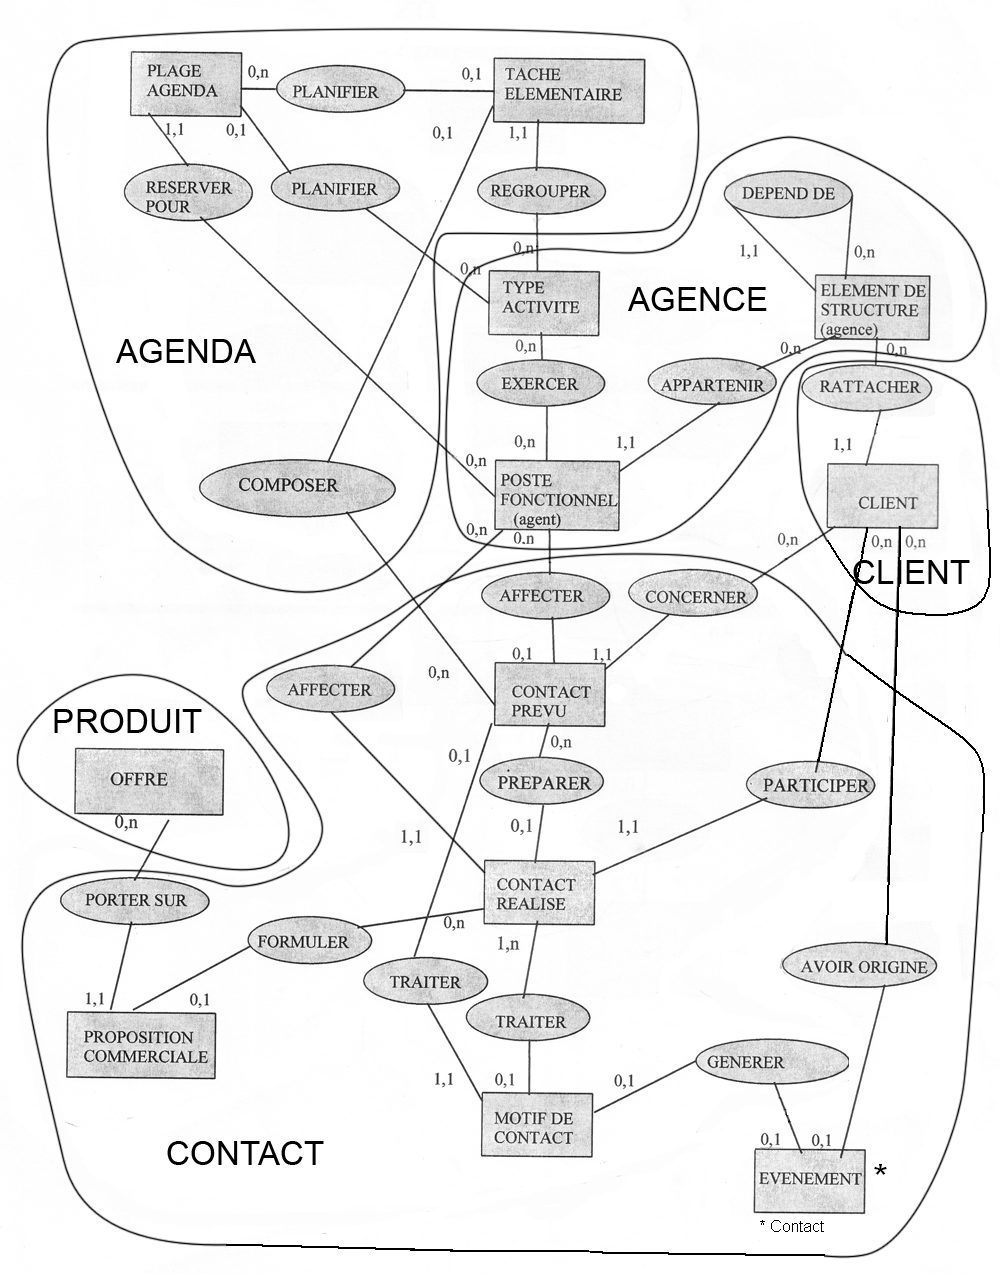
\includegraphics[width=\textwidth]{Decoupage MCD 2.png}
\end {center}

\subsection{Cycles de vie des objets métiers}

Voici le diagramme d'état de l'objet ``Contact'' :

\begin {center}
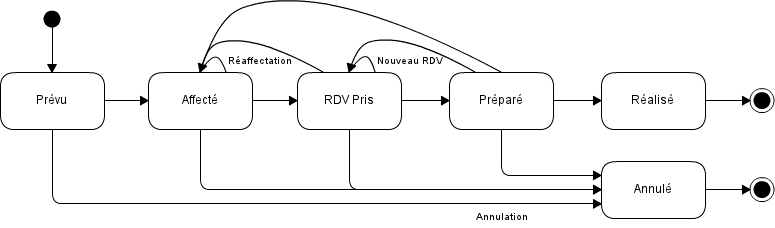
\includegraphics[width=\textwidth]{diagramme-etat-objet-contact.png}
\end {center}
Comme prévu, il n'est pas possible de réaffecter un contact à un autre agent. En effet un agent sera toujours responsable du groupe de contacts qu'on lui a affectés. Néanmoins, les rendez-vous pris, eux, pourront être réaffectés à un autre agent que celui en charge du contact. Cela permettra entre autre de palier à l'absence d'un agent le jour du rendez-vous client.


\subsection{Détermination des flux de l'architecture}

\subsubsection{Diagramme de séquence}

Ci-dessous sont présentés les différents diagrammes de séquences :
\begin {center}
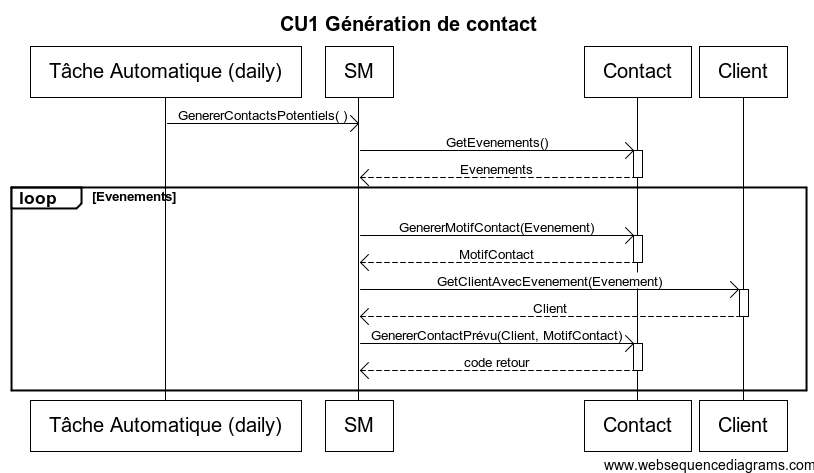
\includegraphics[width=\textwidth]{..\..\webSequenceDiagrameSources\cu1.png}
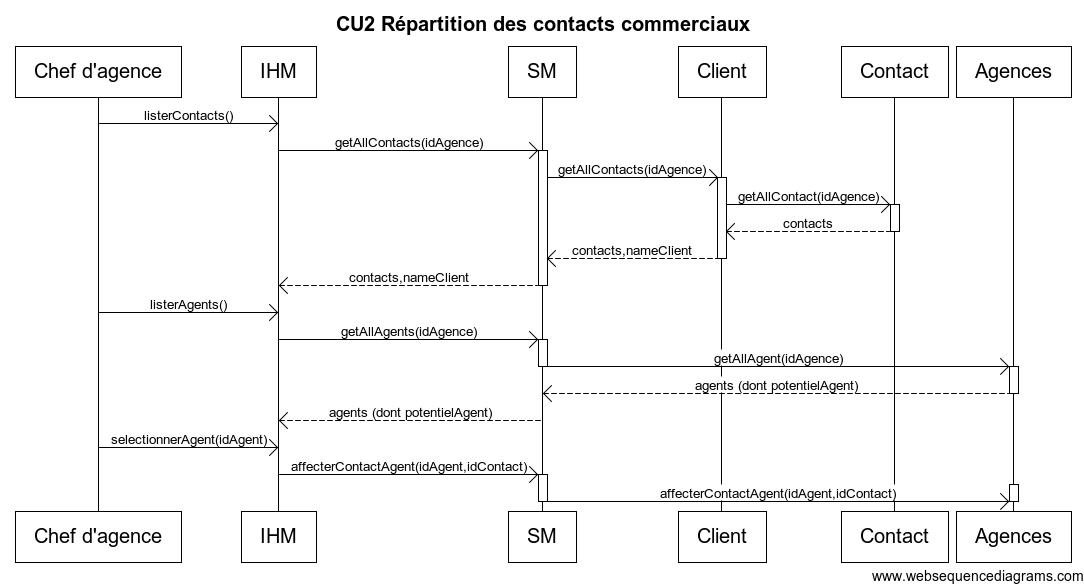
\includegraphics[width=\textwidth]{..\..\webSequenceDiagrameSources\cu2.png}
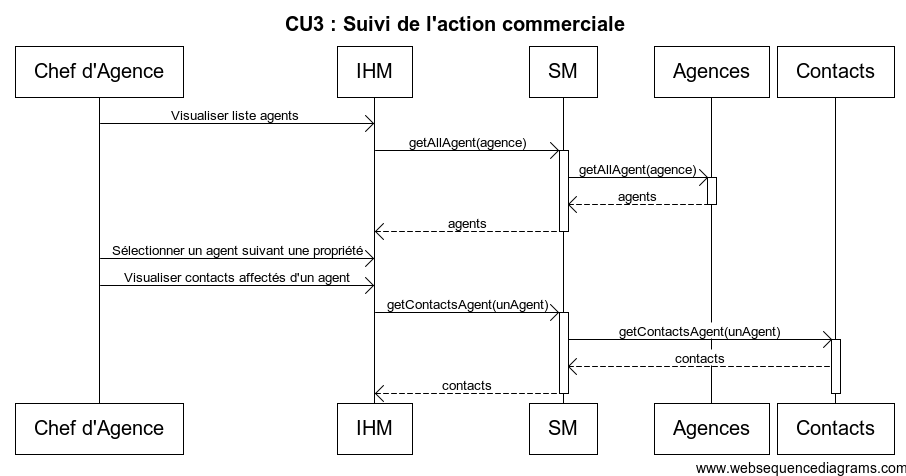
\includegraphics[width=\textwidth]{..\..\webSequenceDiagrameSources\cu3.png}
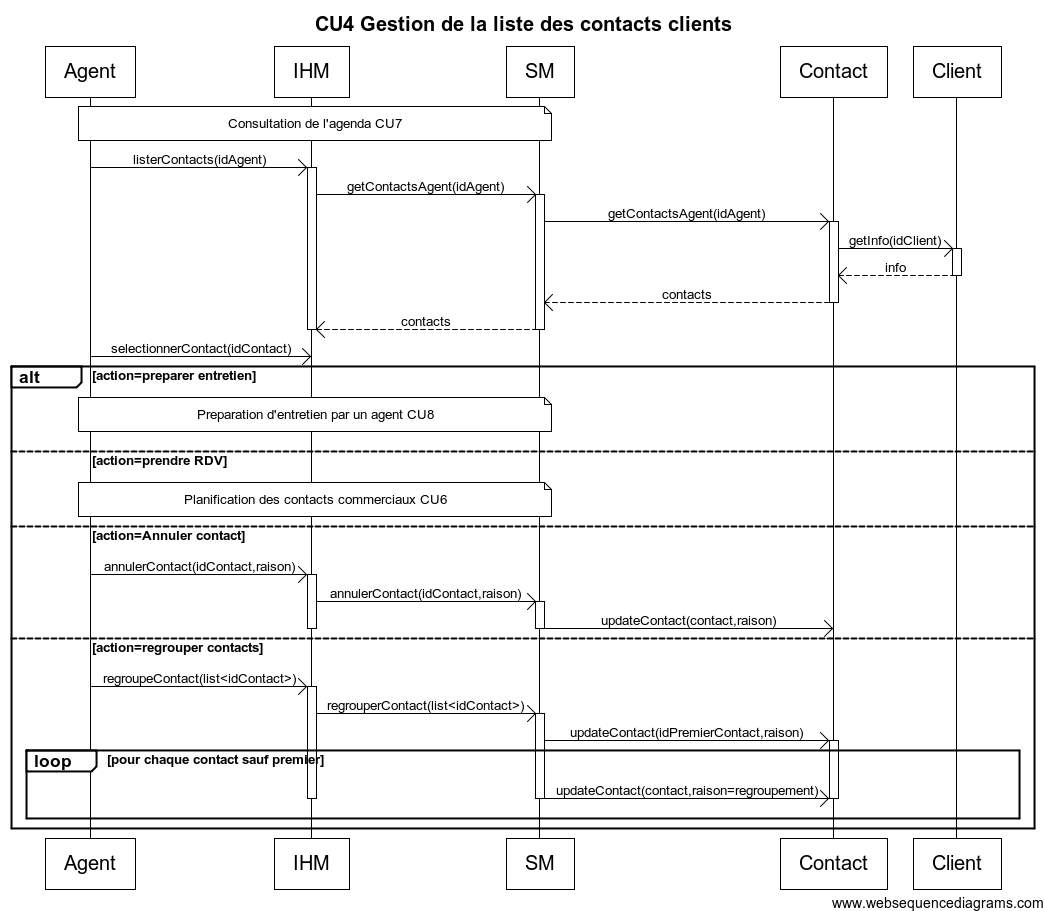
\includegraphics[width=\textwidth]{..\..\webSequenceDiagrameSources\cu4.png}
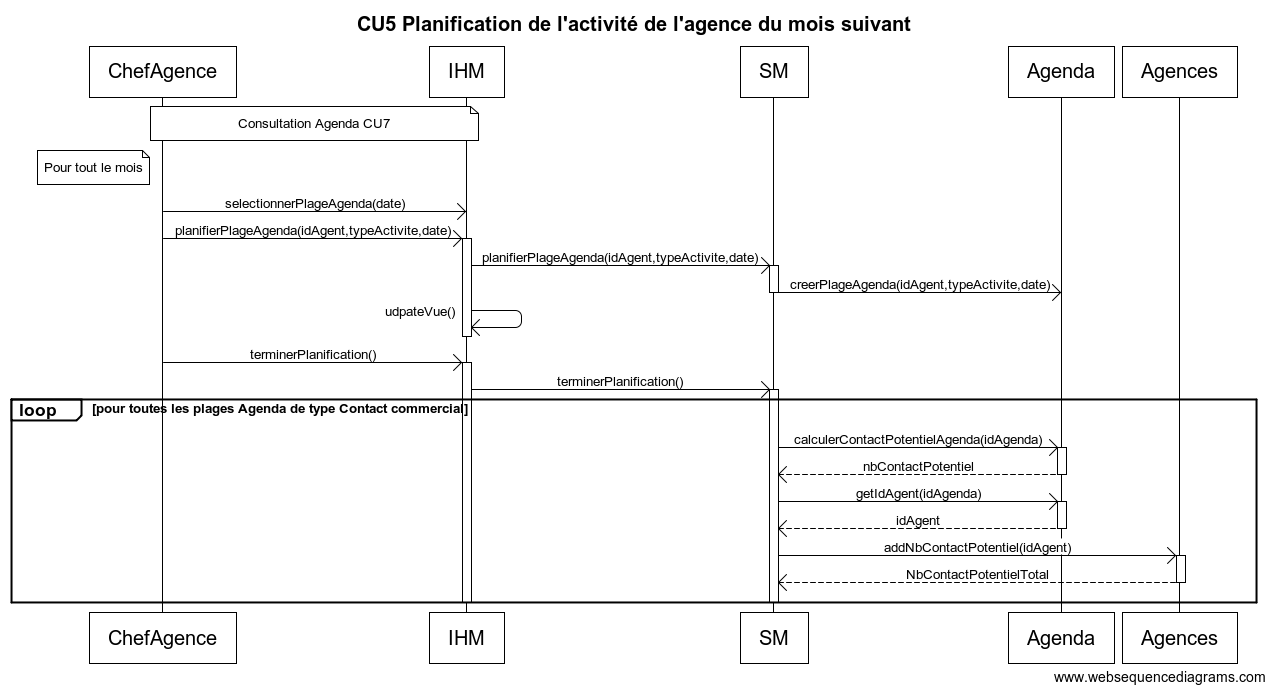
\includegraphics[width=\textwidth]{..\..\webSequenceDiagrameSources\cu5.png}
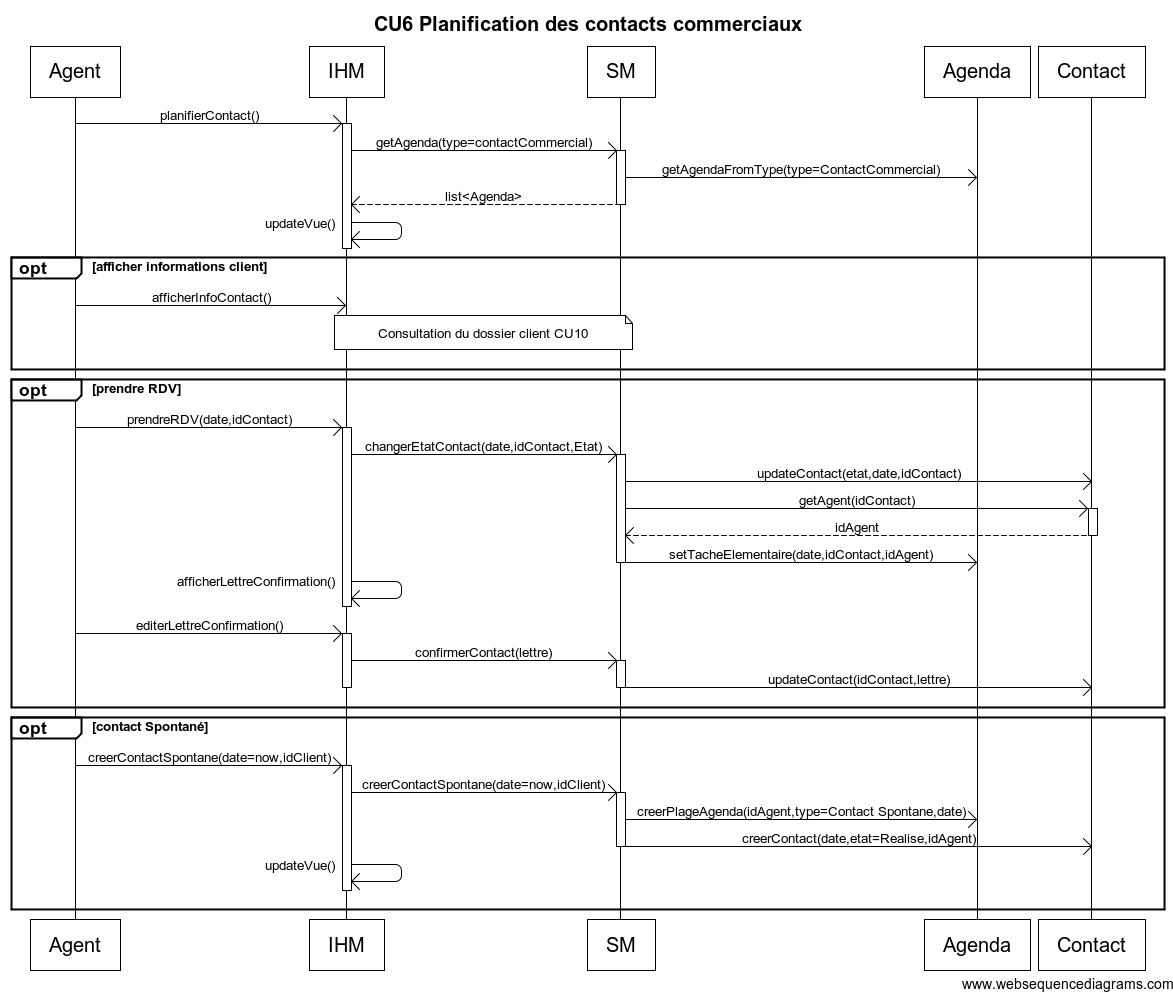
\includegraphics[width=\textwidth]{..\..\webSequenceDiagrameSources\cu6.png}
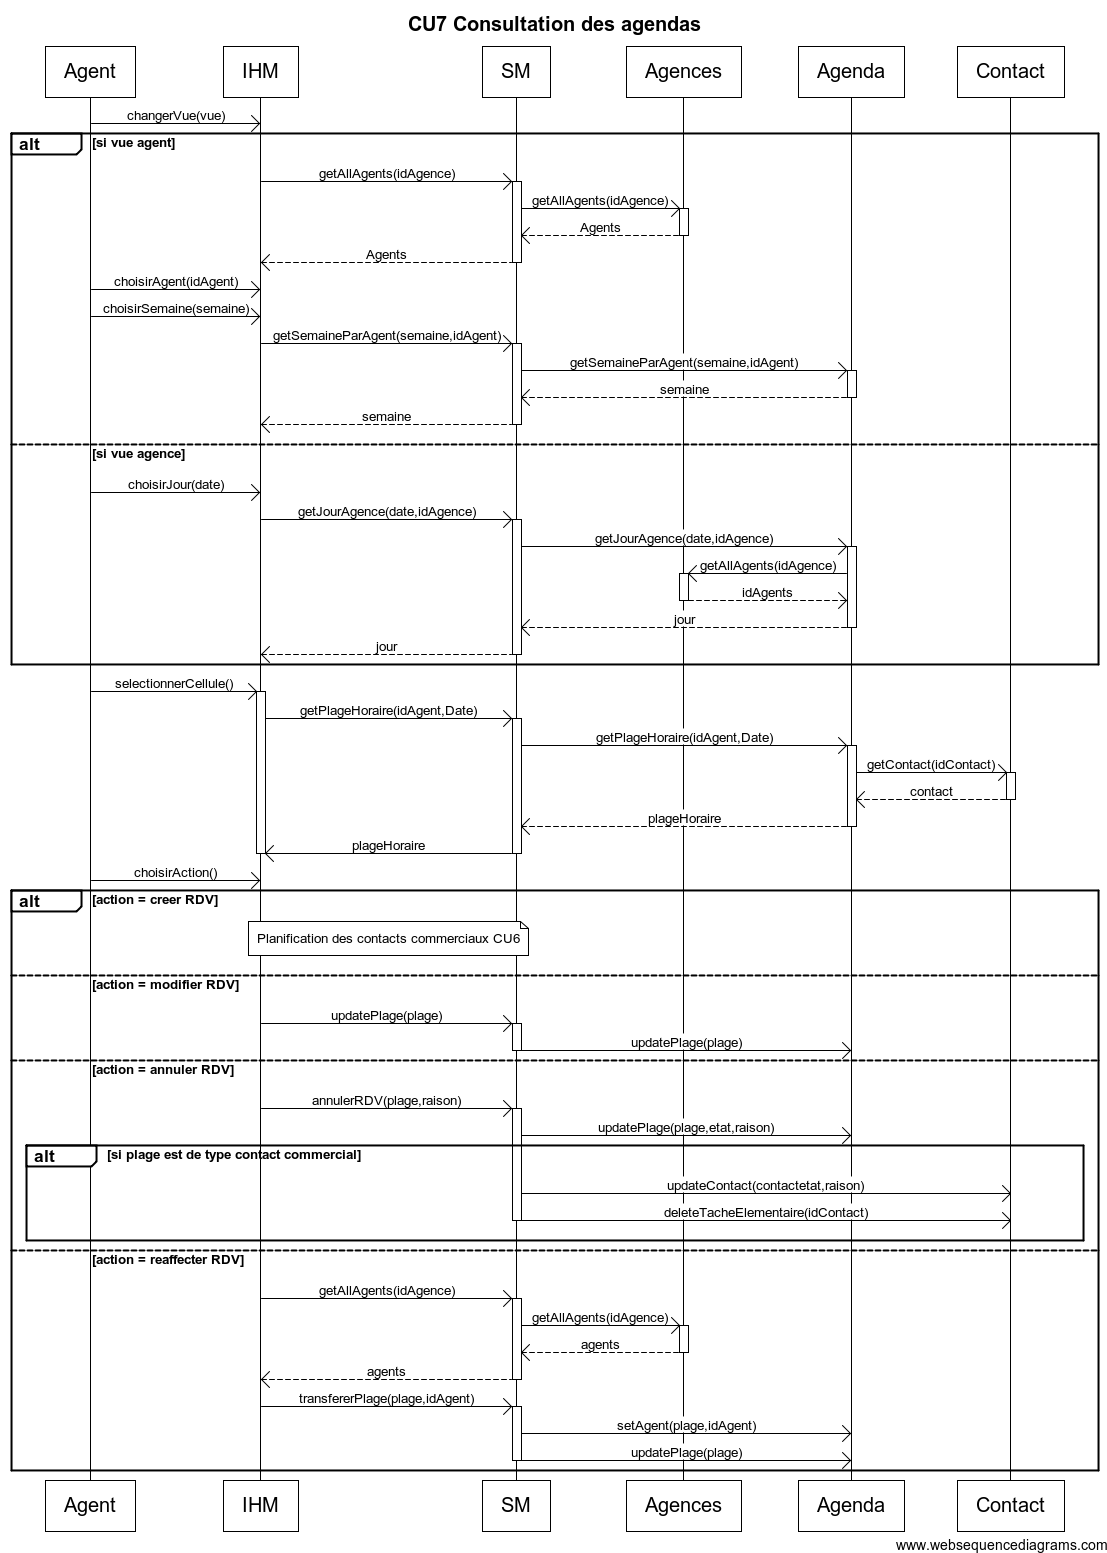
\includegraphics[width=\textwidth]{..\..\webSequenceDiagrameSources\cu7.png}
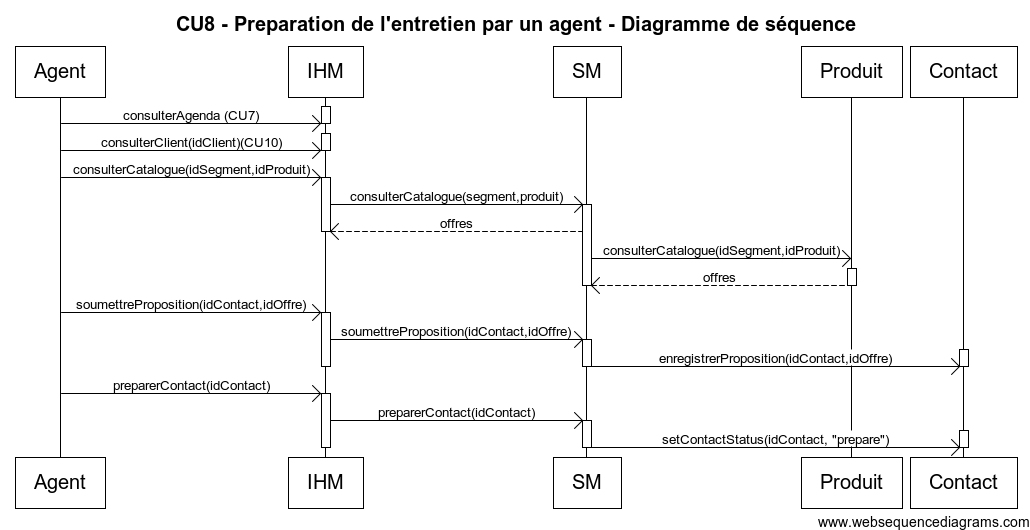
\includegraphics[width=\textwidth]{..\..\webSequenceDiagrameSources\cu8.png}
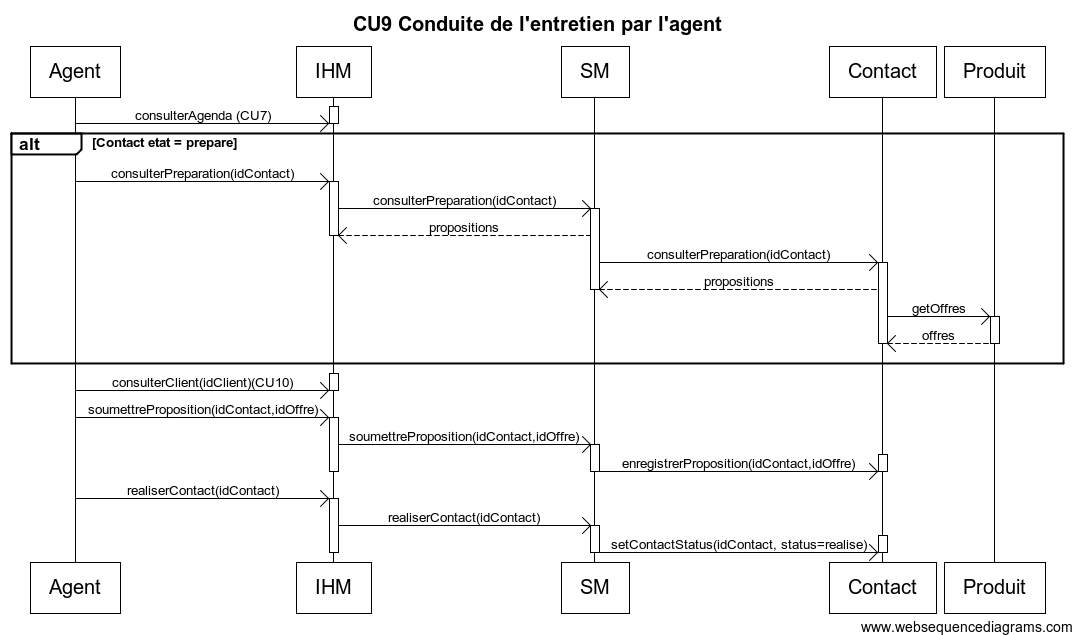
\includegraphics[width=\textwidth]{..\..\webSequenceDiagrameSources\cu9.png}
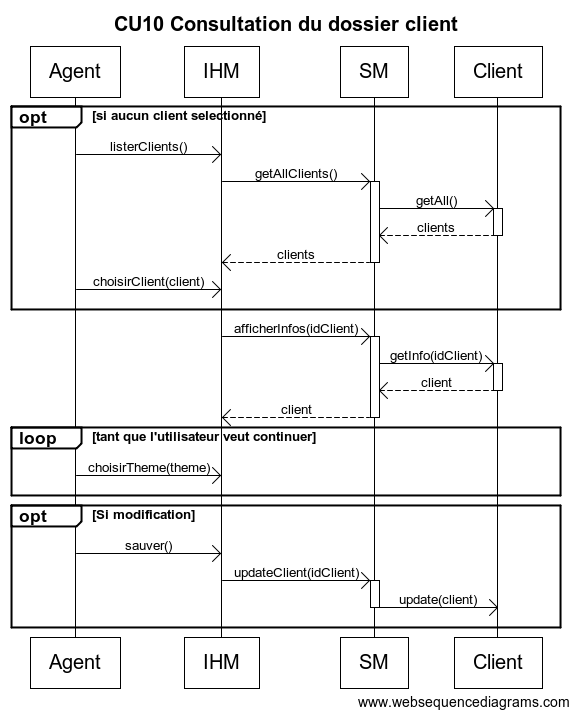
\includegraphics[width=\textwidth]{..\..\webSequenceDiagrameSources\cu10.png}
\end {center}

\subsubsection{Diagramme de collaboration}

Voici le diagramme de collaboration représentatif de la dynamique de
l'architecture:

\begin {center}
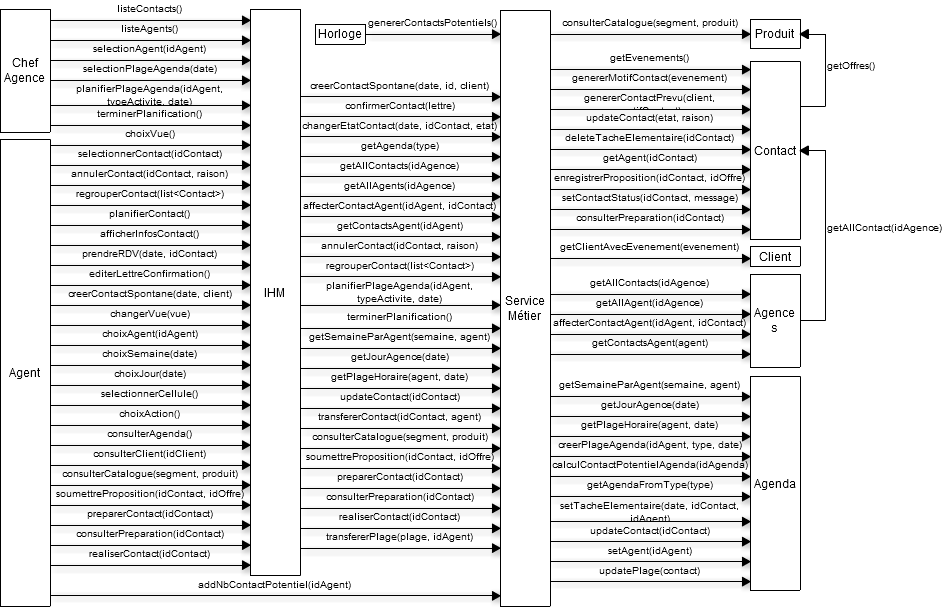
\includegraphics[width=\textwidth]{diagramme-collaboration.png}
\end {center}

Ce diagramme souligne l'existence de flux conséquents entre des groupes de blocs
majeurs, qui permettent d'appuyer le choix de l'architecture retenue, dont nous
discuterons maintenant.


\subsection{Choix de l'environnement technique}
L'environnement technique sera une architecture C/S 3-tiers : l'architecture du système sera donc séparée en trois couches distinctes, à savoir :
\begin{itemize}
\item Couche de données : l'information est stockée ici sur la ou les bases de données. Ces informations seront récuperé par la couche applicative
\item Couche applicative : représente le coeur de l'architecture. A chaque demande de la couche de présentation, la couche applicative va effectuer un calcul, appliquer les règles de gestion et au besoin récuperer les informations de la base de données.
\item Couche de présentation : à chaque action de l'utilisateur, cette couche va d'une part transférer l'information créée par l'utilisateur à la couche applicative et d'autre part afficher l'information récupérée et traitée depuis la base de données par les deux couches précédentes.
\end{itemize}
Le détail de ces tiers sera présenté dans le chapitre 'Architecture technique', notamment la localisation et la répartition des données.

%Corps du document :
%\setlength{\parindent}{1cm}    

\section{Conception détaillée}

Attachons nous maintenant à la conception détaillée de notre application. Il s'agit
d'identifier et de spécifier les composants nécessaires pour automatiser tout ou
partie des outils à utiliser dans le cadre des cas d'utilisation identifiés.

Commençant par spécifier l'enchaînement des fenêtres grâce à un diagramme.

\subsection{Diagramme d'enchaînement des fenêtres}

\begin {center}
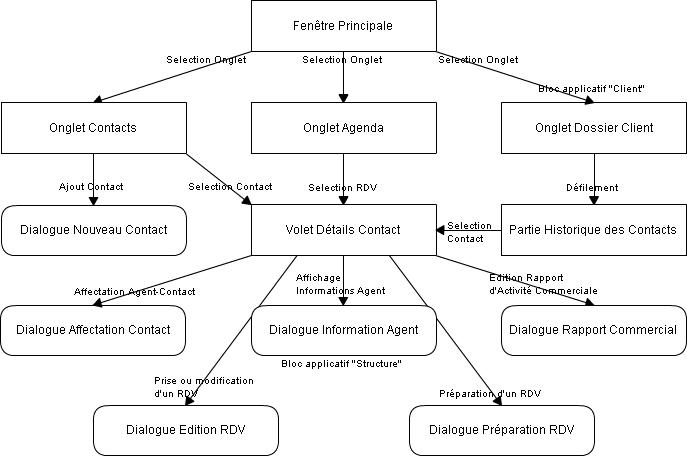
\includegraphics[width=\textwidth]{diagramme-edf.png}
\end {center}

\paragraph{Description}

L'Interface Homme-Machine (IHM) sera composée de trois onglets
principaux :

\begin{itemize}
\item \textbf{L'onglet Contacts} : Il présente la liste des Contacts prévus et affectés.
\item \textbf{L'onglet Agenda} : Il permet de consulter la liste des RDV pris.
\item \textbf{L'onglet Clients} : Cet onglet permet d'accéder aux dossiers des clients de la banque.
\end{itemize}

On observera également le volet \textbf{Détails du Contact}. Il permet d'effectuer toutes les
opérations nécessaires sur un Contact (une liste de ces services métiers se trouve plus loin
dans ce compte rendu).

\subsection{Dessin des fenêtres de l'IHM}

Voici une première représentation graphique de l'IHM que nous contruirons :

TODO @quentez

\subsection{Services Métiers invoqués par l'IHM}

Cette IHM utilise différents services métiers. En voici la liste :

\subsubsection{Services Métier Client}

\paragraph{Recherche de Clients}

\begin{itemize}
\item getAllClients()
\end{itemize}

\paragraph{Dossier Client}

\begin{itemize}
\item afficherInfos(idClient)
\item updateClient(client)
\end{itemize}

\subsubsection{Services Métier Agenda}

\begin{itemize}
\item getAgenda(type)
\item getSemaineParAgent(semaine,idAgent)
\item getJourAgence(date)
\item getPlageHoraire(idAgent,date)
\item planifierPlageAgenda(idAgent,typeActivite,date)
\item terminerPlanification()
\end{itemize}

\subsubsection{Services Métier Contact}

\paragraph{Recherche de Contacts}

\begin{itemize}
\item getAllContacts(idAgence)
\end{itemize}

\paragraph{Affectation des Contacts}

\begin{itemize}
\item getAllAgents(idAgence)
\item getContactsAgent(idAgent)
\item affecterContactAgent(idAgent,idContact)
\item transférerContact(idContact,idAgent)
\end{itemize}

\paragraph{Gestion d'un Contact}

\begin{itemize}
\item updateContact(contact)
\item annulerContact(idContact,raison)
\item changerEtatContact(date,idContact,etat)
\item confirmerContact(lettre)
\item réaliserContact(idContact)
\item regrouperContacts(liste<Contact>)
\item créerContactSpontané(date,idClient)
\end{itemize}

\paragraph{Préparation de l'entretien}

\begin{itemize}
\item consulterCatalogue(idSegment,idProduit)
\item préparerContact(idContact)
\item consulterPréparation(idContact)
\end{itemize}

\paragraph{Rapport d'activité commerciale}

\begin{itemize}
\item soumettreProposition(idContact,idOffre)
\item soumettreRapport{iContact,rapport}
\end{itemize}

\subsection{Spécification des Services Métier}

On ne détaillera que la liste des Services Métier invoqué par l'IHM dossier Client:

SM1: afficherInfo
\begin{itemize}
	\item SOM invoqués : SOMC3 : Consultation informations client
	\item Entrées : idClient
	\item Sorties : NomClient, Adresse, Comptes,....
	\item Procédure :
	\begin{itemize}
		\item Rechercher les informations le client (personne,compte): SOMC5.
	\end{itemize}
\end{itemize}

SM2 : updateClient
\begin{itemize}
	\item SOM invoqués : SOMC4 : Mise à jour des informations client
	\item Entrées : NomClient/Adresse/Compte/... (uniquement ceux modifiées)
	\item Sorties : null
	\item Procédure :
	\begin{itemize}
		\item Mettre à jour les informations sur le client (personne,compte): SOMC4.
	\end{itemize}
\end{itemize}

\subsection{Spécification des Services Objets Métier}

On ne détaillera que les Services Objets Métier concernant le bloc Client:

OM Client SOMC1 : getAllContacts
\begin{itemize}
\item Entrées : idAgence
\item Sorties : liste de (contact, nom du client, adresse client)
\item Entités/Classes : Client - Personne - Adresse - Contact
\item Permet de recuperer tous les contacts non assignés à un agent. Pour cela, la fonction récupère tous les clients de l'agence et verifie si un contact est prévu. 
\end{itemize}

OM Client SOMC2 : genererContactPrevu
\begin{itemize}
\item Entrées : evenement
\item Sorties : idClient
\item Entités/Classes : Evenement - Client
\item La fonction permet de récupérer l'id du client qui est à l'origine de l'évenement.
\end{itemize}

OM Client SOMC3 : getInfo
\begin{itemize}
\item Entrées : idClient
\item Sorties : NomClient, Adresse, Comptes,...
\item Entités/Classes : Client, Personne, Adresse, Compte
\item Permet de consulter toutes les informations d'un client.
\end{itemize}

OM Client SOMC4 : updateInfo
\begin{itemize}
\item Entrées : idClient, info
\item Sorties : null
\item Entités/Classes : Client, Personne, Adresse, Compte
\item Permet de mettre à jour des informations sur un client.
\end{itemize}

OM Client SOMC5 : getAll
\begin{itemize}
\item Entrées : null
\item Sorties : liste Client: NomClient, Adresse,...
\item Entités/Classes : Client, Personne, Adresse, Compte
\item Permet de consulter la liste de tous les clients.
\end{itemize}
%Corps du document :
%\setlength{\parindent}{1cm}    

\section{Répartition des composants sur l'architecture n-tiers}

\subsection{Répartition des blocs applicatifs}

Les blocs \textbf{Produits}, \textbf{Client} et \textbf{Agence} seront implémentés sur le serveur du site central, mais également répliqués sur les serveurs des agences principales. L'architecture de ces données sera en \textbf{multi-maître}. Ainsi, chaque site pourra modifier les données. La gestion des conflits se fera si possible automatiquement, puis au besoin par l'intervention d'un responsable sur le site central.

Les blocs \textbf{Agence} et \textbf{Client}, en plus d'être répliqués, seront répartis. La base de données de chaque agence contiendra seulement les informations des sous-agences qu'elle gère.

Même si les modifications de \textbf{Client} sont nombreuses, peu de conflits seront générés car peu de modifications seront émises à partir du site central. L'intérêt de cette réplication est la sauvegarde des données du client, et un accès aux données accéléré.

Les blocs \textbf{Agenda} et \textbf{Contact} seront répartis. Aucune information ne sera sur le site central. Chaque agence principale gèrera ces propres informations.

\begin {center}
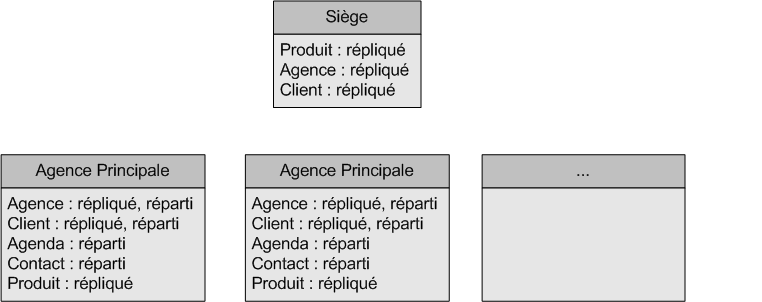
\includegraphics[width=\textwidth]{repartition_bloc.png}
\end {center}

\subsection{Principaux flux applicatifs échangés}

\subsubsection{Consultation des données}

Lorsqu'une donnée est requise par l'une des agences, elle tente si possible de la récupérer sur ses
propres serveurs, ou émet une requète à l'agence principale à laquelle elle est affectée. Celle-ci
peut soit posséder cette donnée, soit la demander au site central, et la mettre en cache. Les systèmes
de cache sont très régulièrement rafraichis afin d'éviter de travailler sur des données trop anciennes
de minimiser le plus possible le risque de conflits (voir les mécanismes de réplication ci-après).

\subsubsection{Mise à jour des données}

\paragraph{Mise à jour active}

Lorsqu'une donnée est mise à jour sur les serveurs d'une agence, et que ces derniers connaissaient les
agences sur lesquelles la donnée est répliquée, ils émettent directement une notification pour les
prévenir du changement.

\paragraph{Mise à jour passive}

Lorsqu'un serveur ne sait pas où se trouvent toutes les copies de ses données, un mécanisme de mise à
jour passive des données intervient. Toutes les données répliquées sont brassées régulièrement,
et transférées de manière routinière entre les agences pour que le système maintienne sa cohérence au
mieux possible tout en veillant à ne pas surcharger le réseau inter-agences.

\subsubsection{Réplication des données}

Pour une plus grande rapidité d'accès, les données considérées comme globales sont répliquées entre les
agences. Elles sont mises à jour le plus régulièrement possible pour garantir la fraîcheur des données
et limiter les risques de conflits.

\paragraph{Réplication descendante}

Comme indiqué précédemment, les données des blocs \textbf{Produits}, \textbf{Client} et \textbf{Agence}
sont répliquées depuis le site central vers les serveurs des agences principales.

\paragraph{Réplication montante}

Il existe également un mécanisme de réplication des données des agences principales vers le site central,
afin que celui-ci puisse conserver des sauvegardes globales (voir paragraphe suivant). De la même façon,
les sous-agences répliquent leurs données vers les agences principales auxquelles elles sont affectées.
Cette réplication montante ne concerne pas les blocs applicatifs \textbf{Agenda} et \textbf{Contact}, car
ils relèvent de la responsabilité des sous-agences seules.

\subsubsection{Sauvegarde des données}

Les données sont systématiquement et régulièrement sauvegardées.

\paragraph{Restauration intégrale à froid}

Celles qui sont présentes ou répliquées
sur le site central sont enregistrées sous forme de clichés instantanés, qui peuvent être restaurés
intégralement à froid en cas de problème majeur (cas extrêmes comme la perte d'un ou plusieur serveurs).

\paragraph{Restauration partielle localisée à chaud}

Un mécanisme de restauration partielle à chaud est également prévu pour
les problèmes de pertes de données localisées, comme la perte d'un dossier ou la corruption d'une entrée
au sein d'une base de données. Ce mécanisme est géré automatiquement par notre système de Base de Données.

Il existe des systèmes de sauvegardes similaires au sein de chaque agence.

%----------------------------------------------------

\end{document}
